\documentclass{article}


%\usepackage{nips_2017}

% to compile a camera-ready version, add the [final] option, e.g.:
\usepackage[final]{nips_2017}

\usepackage[utf8]{inputenc} % allow utf-8 input
\usepackage[T1]{fontenc}    % use 8-bit T1 fonts
\usepackage{hyperref}       % hyperlinks
\usepackage{url}            % simple URL typesetting
\usepackage{booktabs}       % professional-quality tables
\usepackage{amsfonts}       % blackboard math symbols
\usepackage{nicefrac}       % compact symbols for 1/2, etc.
\usepackage{microtype}      % microtypography
\usepackage{graphicx}
\graphicspath{{images/}}
\title{Rap Machine}



\author{
  De Huo \\ \texttt{dhuo@ucsc.edu} \\ \And
  Ke Wang \\ \texttt{kwang82@ucsc.edu} \\ \And
  Nursultan Kabylkas \\ \texttt{nkabylka@ucsc.edu} \\ \And
  Ramesh Jayaraman \\ \texttt{rkjayara@ucsc.edu} \\ \And
  Yuan Yang \\ \texttt{yyang175@ucsc.edu} 
}

\begin{document}

\maketitle

\begin{abstract}
We present Rap Machine, an image based lyrics generator. We use a CNN model extract features from images, caption the image using a RNN model, and generate lyrics in the style of an artist using a sequence to sequence model. We train and evaluate our image captioning model using the Flickr 8k dataset, and use lyrics from several artists across different genres and writing styles to train and generate lyrics based on the caption we obtained from the image captioning model.
\end{abstract}

\section{Introduction}

We are proposing to combine image captioning implemented with Convolution
Neural Nets and poem generation implemented with Recurrent Neural Nets.
The idea is to train CNN to caption images with sentences, and also train RNN
with the song lyrics of different famous artists, such as: 2Pac, 50 cent, Eminem, Coldplay, Tool, Iron Maiden etc.

Once the two Neural Net models are trained, we will use a test set of images
to generate image caption, using the CNN model, and feed the generated text as
an input of the RNN model, to generate the Poem/Lyrics. The purpose of this
project is to evaluate the performance of RNN model, and compare generated
lyrics among different artists, so as to compare their ”style” of writing.

We will first provide details about our implementation of image captioning in section \ref{sec:2}, followed by  our implementation of lyrics generation in section \ref{sec:3}. We will then present our evaluation, combining the models together in section \ref{sec:4}, and conclude our work in section \ref{sec:5}.

\section{Image Captioning}
\label{sec:2}
Image captioning is the process of generating textual descriptions of images. It mainly consists of two parts, image features extraction parts using CNNs and textual descriptions generating parts using RNNs. Training a CNN network costs huge amount of time and requires a super large data pool. So based on our limitations, we implemented a well trained CNN model for our image extraction, it is InceptionV3. After we got the image features, we merged the image’s feature and the word’s feature together and feed it into a bidirectional RNN to caption our image. 

\begin{figure}[!ht]
\centering
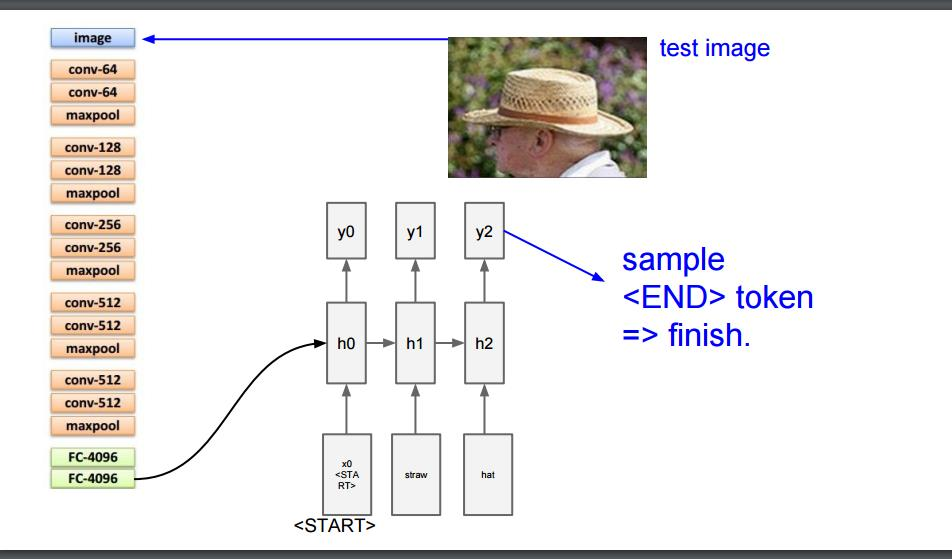
\includegraphics[scale=0.30]{1.png}
\caption{Architecture of the proposed implementation}
\label{fig:1}
\end{figure}

\subsection{Image Feature Extraction}

Convolutional Neural Networks is the most commonly used network to process images. After the great breakthrough made in 2012, “AlexNet”, a few well performed CNN models came, such as “GoogleLeNet” and “InceptionV2”. They were all focusing on improving the functional performance of the single convolutional module.  InceptionV3 is a more advanced CNN model to process the image. It factorizes the two dimensional convolutional layer to two one dimensional convolutional vectors for accelerating the calculating speed and increasing the networks’ depth \ref{ref:1}
	Inception V3 model can classify images into 1000 classes with high accuracy and high computational efficiency. Therefore, we used pre-trained inception V3 model to obtain features of images.

\subsection{Textual Descriptions Generation}
\begin{figure}[!ht]
\centering
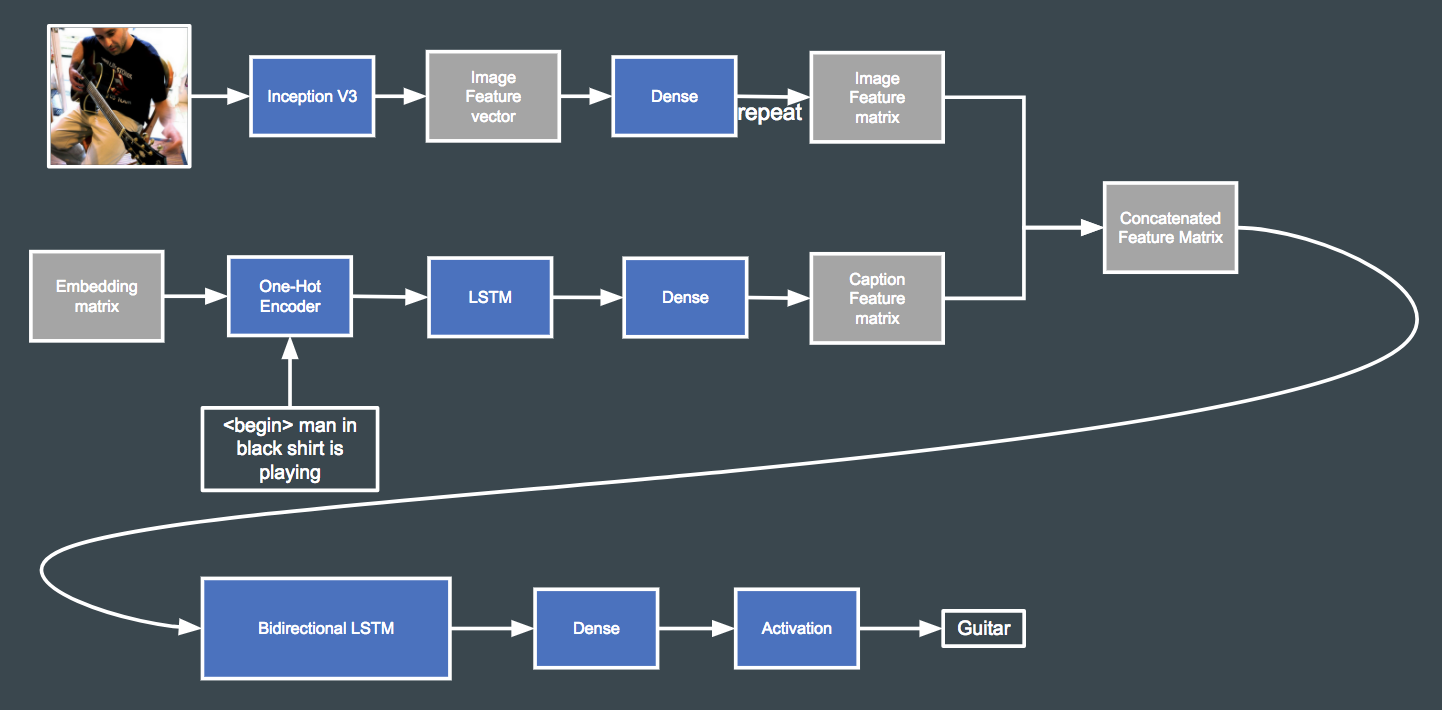
\includegraphics[scale=0.26]{2.png}
\caption{Architecture of our image captioning model}
\label{fig:2}
\end{figure}
\subsubsection{Architecture}
We feed one picture into InceptionV3 model, then the CNN will give us a feature vector of that picture after processing it. The dimension of the image feature vector is 2048. We don’t want to train too many parameters in RNN model, because it costs too much time. So we compact the dimension to 256, and let it repeat 40 times, which is the max length of our text sentences. And now we get a single image matrix (256 x 40).

We let the model train the word embedding matrix with dimension 256 , and we use the One-Hot matrix which generates from each description sentences for a picture to look up a word feature matrix (256 x 40). Then we sent the matrix to a LSTM RNN for training the embedding matrix. Another purpose of this LSTM is to get the sentence’s feature for each word in this sentence. The dimension of this matrix is also 256 x 40, and we call it Caption feature matrix.  

We concatenate Image feature matrix and Caption feature matrix into a concatenates feature matrix with size 600 x 40. Let it be the input of Bidirectional LSTM and output a feature vector of the generated word (1 x 512), using a dense layer to transfer the size to 1 x 8000. At last, using softmax activation layer to obtain the vector that represents the generating word.

When training, the input is the image and the front part of the sentence which includes the words that have already generated before. The output is the next word of the input uncompleted sentence. Training of one sentence halt once output is “<end>”.

\subsubsection{Dataset}

In general, datasets for image captioning include images and some captions that describe these images. There are several datasets for image captioning, such as Flickr 8k, Flickr 30k, Microsoft COCO, UIUC Pascal Sentence and so on. Because of limitations of time and training environments, we chose Flickr 8k as our dataset since it has relatively small size comparing to Flickr 30k and Microsoft COCO, and more images and sentences comparing to Microsoft COCO. Flickr 8k dataset contains 6000 training images, 1000 validation images and 1000 test image with 5 textual descriptions of each image. 21\% images have static verbs like sit, stand, wear, look or no verbs.

\subsubsection{Hyperparameters}

The optimizer of our model is the Adam optimizer. The parameter of Adam optimizer comes from its original paper[2].  
Convergence of Adam is quite fast compares to other methods. The Loss function we chose is the softmax cross entropy loss. The training batch size we chose is 256. 

\subsection{Image Captioning Results}

After 100 epochs training, our loss reached 2.016 and we got a training accuracy of 0.501. One of test results is shown in Figure \ref{fig:3}. 

\begin{figure}[!ht]
\centering
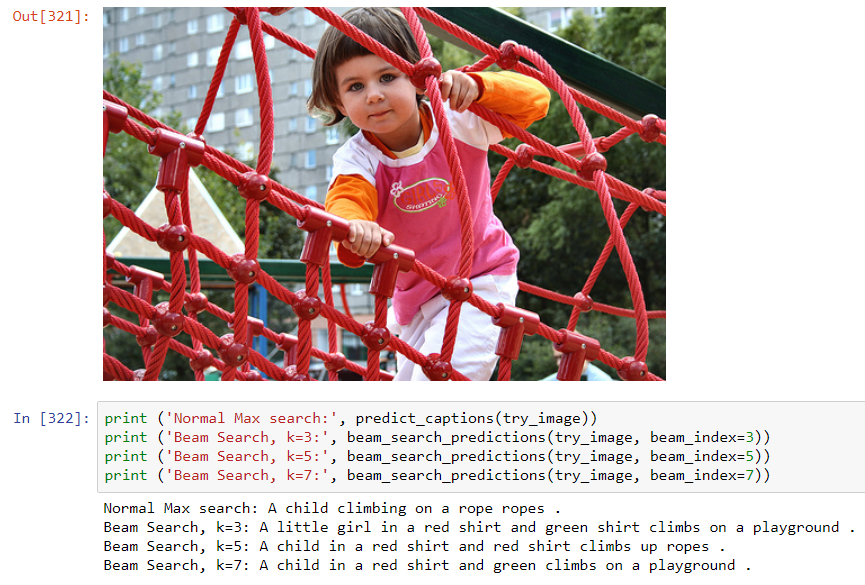
\includegraphics[scale=0.65]{3.png}
\caption{Architecture of the proposed implementation}
\label{fig:3}
\end{figure}

\section{Lyrics Generation}
\label{sec:3}

\subsection{Background}
For lyrics generation we decided to use encoder-decoder model. This model typically is used for Neural Machine Translation(NMT). Figure \ref{fig:encdec-model} depicts the model in action. First, a sentence in source language is fed into the encoder, which in turn generates a feature vector. This feature vector sometimes referred to as a "thought vector" due to the fact that the value of the vector carries a semantic meaning of the source sentence. Lastly, the thought vector is passed into the decoder, which after the processing spits out the sentence with the same meaning but in a target language.\\
\begin{figure}[!ht]
\centering
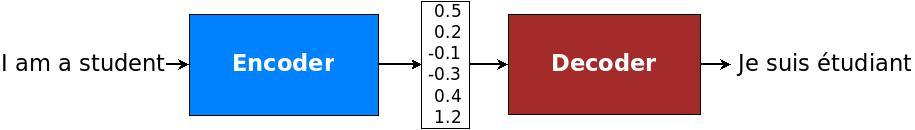
\includegraphics[scale=0.4]{encdec.jpg}
\caption{Encoder-decoder model}
\label{fig:encdec-model}
\end{figure}

Although the design of the encoder and decoder may vary, the typical implementation is shown in Figure \ref{fig:nmt-arch}. Because of the sequential nature of the data, i.e. human language the RNN is used for both encoder and decoder. The type of the RNN (vanillaRNN, LSTM, GRU, etc.) must be chosen based on the application. In Figure \ref{fig:nmt-arch} "<s>" represent the start of the decode phase, while </s> signals the stop.
\\
\begin{figure}[!ht]
\centering
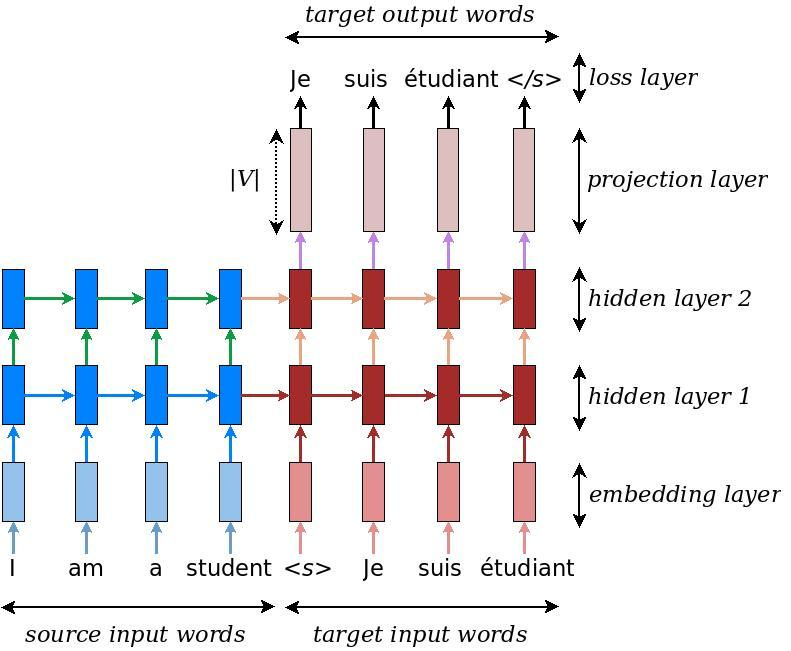
\includegraphics[scale=0.35]{nmt-architecture.jpg}
\caption{Architecture of NMT model}
\label{fig:nmt-arch}
\end{figure}

At this point, a good question to ask is "How all these can be applied to lyrics generation?" Please refer to the Figure \ref{fig:encdec-for-lyr}. For instance, let's consider two lines of lyrics. Line 1: "Guess who's back?" Line: "Back again!". By feeding the first line to the encoder part and the second line to the decoder part, we teach the model to generate next line based on what is provided as the previous line. This model was proved to be working by Qixin Wang et al. [cite] This paper was referenced through out the implementation of this project.

\begin{figure}[!ht]
\centering
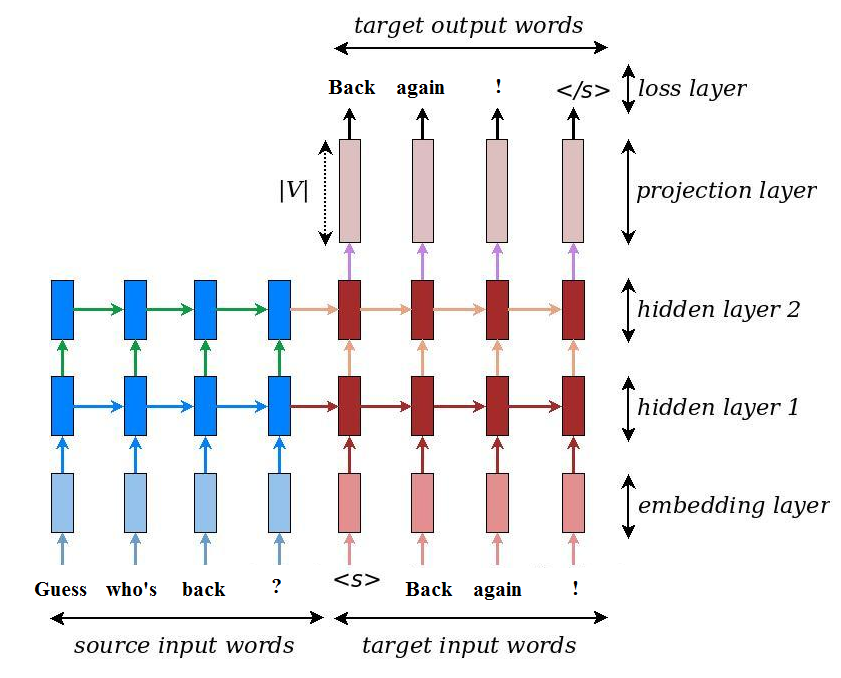
\includegraphics[scale=0.35]{5.png}
\caption{Encoder-decoder model used for lyrics generation}
\label{fig:encdec-for-lyr}
\end{figure}

\subsection{Architecture}
Figure \ref{fig:our-arch} depicts the architecture of the model that we implemented. Table \ref{tab:arch-summary} summarizes the architecture parameters. GRU cell was used for RNN implementation. GRU is similar to LSTM but has simpler "piping" hence performs less calculation. The choice of GRU as a RNN cell was based on the fact that lyrics lines does not need very long term dependence because typical lyric line range from 4 to 15 words. Also, for quick testing purposes we used small dataset, namely, one album of Eminem which is around 1000 lines of lyrics. This resulted in vocabulary size of 2K. Final training was performed on 130K lines of lyrics which resulted in around 30K of unique vocabulary in the dictionary.
\begin{table}[]
\centering
\label{tab:arch-summary}
\begin{tabular}{|l|l|}
\hline
Loss function & sparse\_softmax\_cross\_entropy\_with\_logits \\ \hline
Optimizer     & AdamOptimizer                                 \\ \hline
Learning rate & 0.001                                         \\ \hline
RNN type      & GRU                                           \\ \hline
State size    & 256                                           \\ \hline
Vocab size    & ranged from 2K to 30K                         \\ \hline
\end{tabular}
\caption{Architecture summary}

\end{table}

\begin{figure}[!ht]
\centering
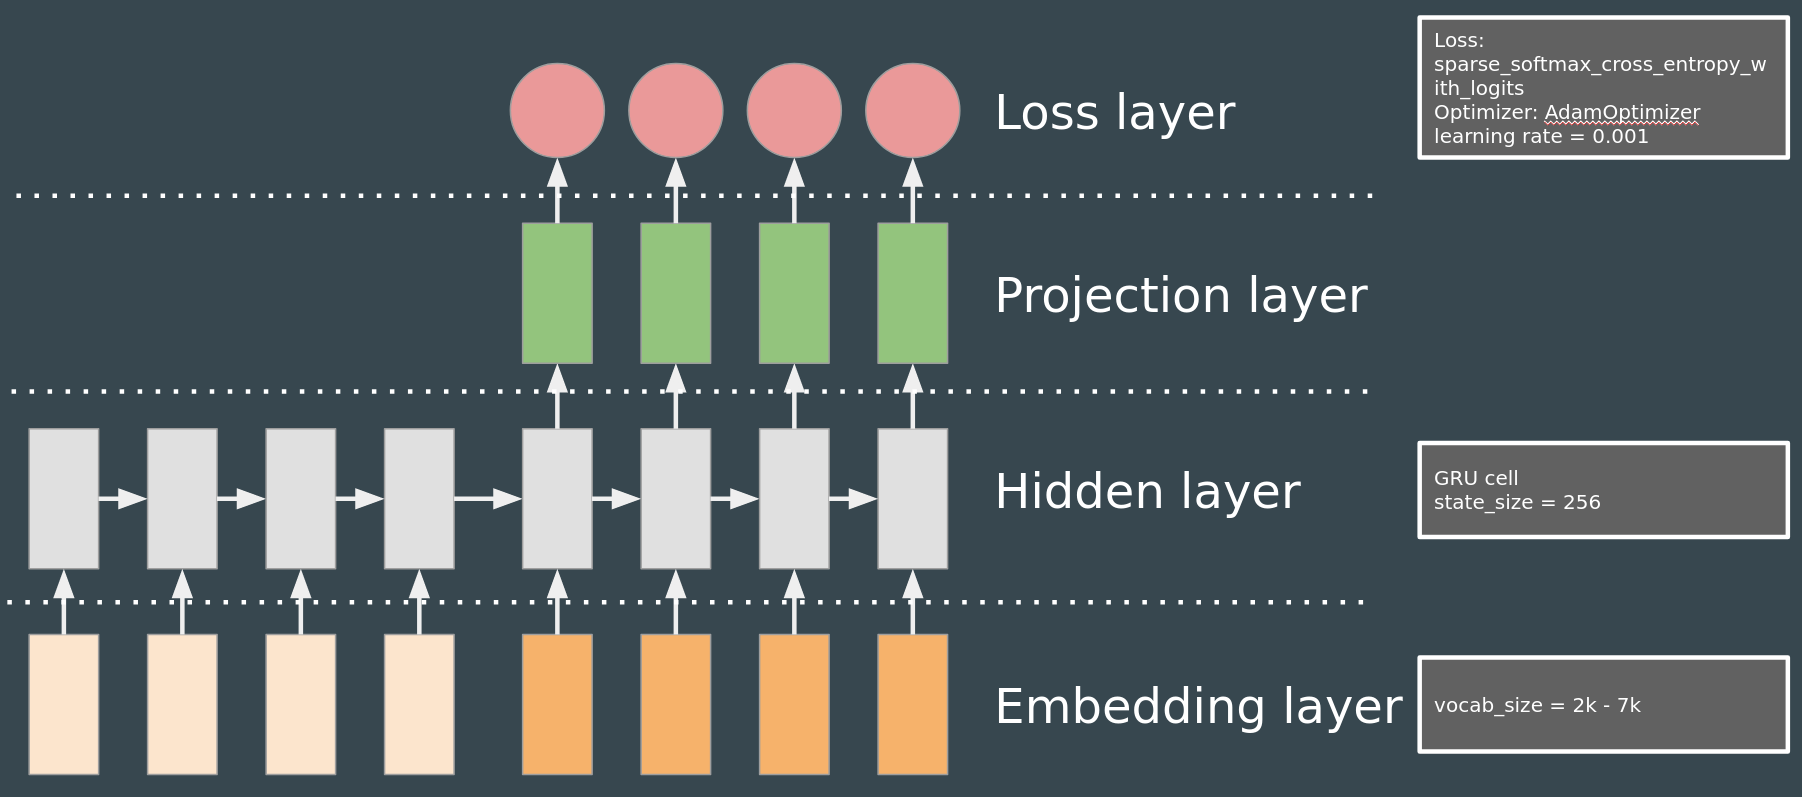
\includegraphics[scale=0.2]{4.png}
\caption{Architecture of our image captioning model}
\label{fig:our-arch}
\end{figure}
\subsection{Dataset}

As we wanted to train the model using different writing styles that different artists follow (a genre/artist specific model), we used a script and scraped our lyrics from AZLyrics [cite]. We then removed repeating lines, abbreviations, and other content that we felt would interfere with the training of our model. We also used the Kaggle 55000+ song dataset [cite] to train and test our model for generalized lyrics generation (as a generic lyrics generation model). We also wanted to use the million song dataset [cite], but we were unable to train and test our model using this dataset due to limited time and computational resources despite using GPUs.

\subsection{Training}
For simplicity reasons and due to the abundance of data we used single split cross validation method. 80\% of the data was randomly taken from the dataset and used for training, while remaining 20\% left for validation. To evaluate the quality of generated lines the "Bilingual Evaluation Understudy" (BLEU) technique proposed by [Papineni et al., 2002] was used. BLEU metric ranges from 0, meaning the generated result is of poor quality, to 1, meaning the result is of high quality, respectively. From Figure \ref{fig:bleu} can be seen that, for validation set, the quality of generated lyrics increase as the training proceeds. Also, Figure \ref{fig:loss} depicts that as the training goes the model learns as the loss on validation set drops.

\begin{figure}[!ht]
\centering
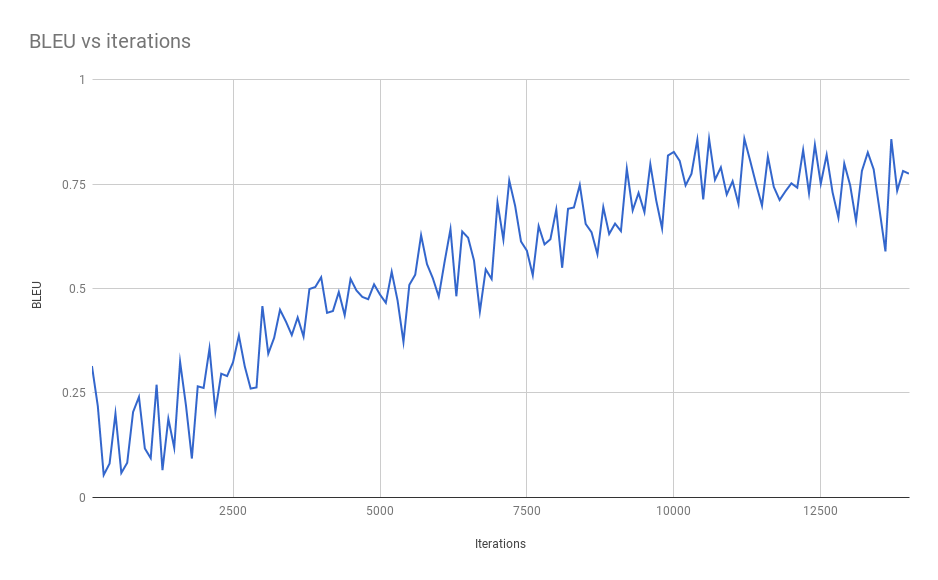
\includegraphics[scale=0.42]{bleu.png}
\caption{Increase in quality of generated lines}
\label{fig:bleu}
\end{figure}

\begin{figure}[!ht]
\centering
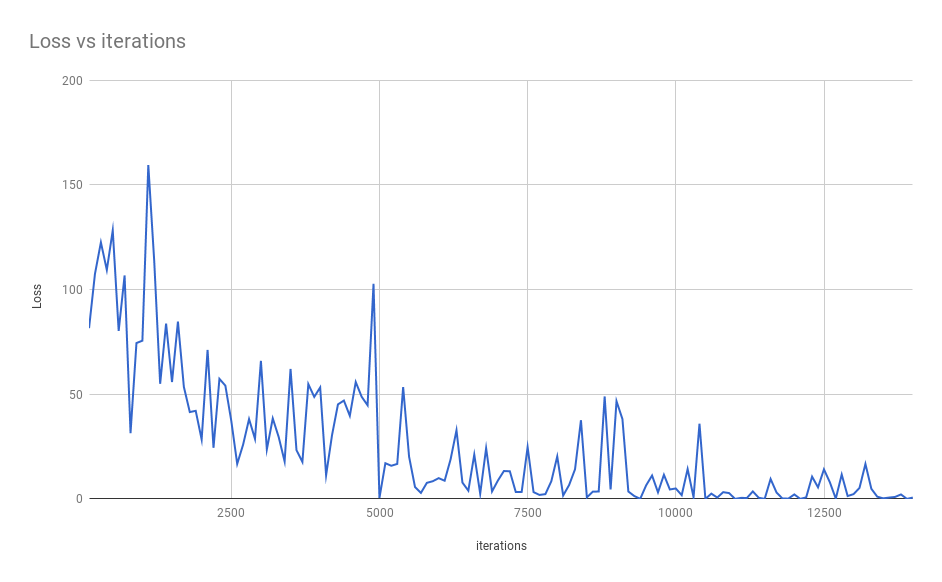
\includegraphics[scale=0.42]{loss.png}
\caption{Decrease in loss on validation set}
\label{fig:loss}
\end{figure}


\subsection{Challenges and Results}
We faced a problem when trying to combine the image captioning and lyrics generation models. The problem is that two models were trained on completely different datasets from completely different domains. The lyrics generation model got confused if it was provided a seed with completely unknown lines. For instance, Table \ref{badresults} how this is happening. For the seed "I love you, dear", which was not in found in the training and which is not the typical phrase used by the artist, the model generated the lines that did not make sense. \\

Here is the solution we found: given the seed, find the closest line in the training set based on the cosine difference. Please refer to [cite] to read more about cosine difference. In a nutshell, cosine finds the similarity between two texts based on the word frequency in that text. By implementing this, we were able to get related to the seed lines in the training set, and let the model generate lyrics from what it had seen. Table \ref{table-transform} shows some examples of this transformation. The last line of Table \ref{table-transform} shows that transformation can give completely irrelevant result. We believe that this can be fixed by increasing the training set since the transformation will have many lines to choose from. \\

Table \ref{tab:betterresult} show the result of the model for the same seed as in Table \ref{tab: bad-results}. It can be seen that the generated lines are not perfect, but they are very relevant.

\begin{table}[]
\centering
\begin{tabular}{l}
\hline
Seed: "I love you, dear"                                    \\ \hline
you’re like an argument over a parking spot                 \\
their front porch , their front porch                       \\
but i ain’t tryna have none of my people hurt and murdered  \\
im supposed to be the soldier who never blows his composure \\ \hline
\end{tabular}
\caption{Generated lines when model sees unknown line}
\label{badresults}

\end{table}

\begin{table}[]
\centering
\label{table-transform}
\begin{tabular}{|l|l|}
\hline
\textbf{Seed}                                           & \textbf{Closest line in training set}                              \\ \hline
I love you, dear                                        & cause you love me, and i love you more                             \\ \hline
A woman with the necklace posing for the camera         & got our name from a woman and our game from a woman                \\ \hline
A man in red vest wakeboarding                          & already in the red                                                 \\ \hline
A child in a red shirt and green climbs on a playground & professor x vanglorious exists in a state of red, black, and green \\ \hline
\end{tabular}
\caption{Transformation of the seed to a familiar lyric line}
\end{table}

\begin{table}[]
\centering
\label{tab:better-result}
\begin{tabular}{l}
\hline
Seed: "I love you, dear"                                        \\ \hline
Transformed seed: "cause you love me, and i love you more"      \\ \hline
You’re , i want you to focus                                    \\
I was gonna take the time to sit down and write you to go,      \\
But i thought thought a song would probably be a little better, \\
Instead of just a letter                                        \\ \hline
\end{tabular}
\caption{Generated lines with transformed seed}
\end{table}

\section{Evaluation}
\label{sec:4}

In this section we provide our evaluation by combining the image captioning and lyrics generation models, and generating lyrics based on the caption generated by our model. 

\section{Conclusion}
\label{sec:5}

We implemented the proposed image captioning based lyrics generation model, and evaluated it using the Flickr 8K dataset and lyrics from several artists. We achieved accurate captioning and lyrics generation for different artists and across artists using the Kaggle 55000+ song dataset.





\end{document}
